\chapter{Аналитический раздел}

В данном разделе проводится анализ предметной области, описание карточек для альтернативного взаимодействия PECS, проводится классификация существующих СУБД. На основе анализа предметной области составляется список пользователей системы, а также создаётся диаграмма вариантов использования, а также диаграмма сущность-связь в нотации Чена. На основе данных, которые будут хранится в системе выбирается модель базы данных.

\section{Понятие базы данных}

\textbf{Определение БД}

Большинство определений понятия <<база данных>> носят субъективный характер и мнение тех или иных авторов.
Однако можно отметить наиболее общие из них.

\textbf{База данных}~\cite{date} --- это некоторый набор перманентных (постоянно хранимых) данных, используемых прикладными программными системами \newline какого-либо предприятия.

\textbf{База данных} --- это самодокументированное собрание интегрированных записей.

\textbf{Типы баз данных}

По типу применения базы данных делятся на:

\begin{enumerate}[label=\arabic*.]
	\item \textbf{OLAP}(online analytical processing) --- это технология обработки данных, которая используется для анализа больших объемов данных.
	\item \textbf{OLTP}(online transactional processing) --- это технология обработки транзакций, которая используется для выполнения операций в режиме реального времени.
\end{enumerate}

В силу необхоимости работать в режиме реального времени для разрабатываемого программного продукта будет выбрана технология OLTP.

\section{Понятие системы управления базами данных}

\textbf{Определение СУБД}

Для взаимодействия с любой базой данных необходима система управления.

\textbf{Система управления базами данных (СУБД)} --- это приложение обеспечивающее создание, хранение, обновление и поиск информации в базе данных.

\textbf{Классификация СУБД}

\textbf{По модели данных}

\begin{enumerate}[label=\arabic*.]
	\item \textbf{Дореляционные}
	\begin{enumerate}[label=\alph*.]
		\item \textbf{Инвертированные списки} (файлы). БД на основе инвертированных списков представляет собой совокупность файлов, содержащих записи (таблиц). Для записей в файле определен некоторый порядок, диктуемый физической организацией данных. Для каждого файла может быть определено произвольное число других упорядочений на основании значений некоторых полей записей (инвертированных списков). Обычно для этого используются индексы. В такой модели данных отсутствуют ограничения целостности как таковые. Все ограничения на возможные экземпляры БД задаются теми программами, которые работают с БД. Одно из немногих ограничений, которое все-таки может присутствовать --- это ограничение, задаваемое уникальным индексом. 
		\item \textbf{Иерархическая модель} данных подразумевает что элементы, организованные в структуры, объединены иерархической или древовидной связью. В таком представлении родительский элемент может иметь несколько дочерних, а дочерний --- только один родительский.
		\item \textbf{Сетевые} --- могут быть представлены в виде графа; логика выборки зависит от физической организации данных.
	\end{enumerate}
	\item \textbf{Реляционные}
	
	В отличие от дореляционных, в данной модели не существует физических отношений между сущностями. Хранение информации осуществляется в виде таблиц (отношений), состоящих из рядов и столбцов.  Отношение имеет имя, которое отличает его от имён всех других отношений.
	\begin{enumerate}[label=\alph*.]
		\item \textbf{Структурные} --- данные --- набор отношений.
		\item \textbf{Целостностные} --- отношения (таблицы) отвечают определенным условиям целостности.
		\item \textbf{Манипуляционные} --- манипулирования отношениями осуществляется средствами реляционной алгебры и/или реляционного исчисления.
	\end{enumerate}

\item \textbf{постреляционные~\cite{vinograd}}

	Основным недостатком реляционных баз данных является ограничение поддерживаемых типов. Большинство постреляционных баз данных основаны на хранении данных в виде сложных структур.
	\begin{enumerate}[label=\alph*.]
		\item \textbf{Объектные} --- данные моделируются в виде объектов;
		\item \textbf{Объектно-реляционные} --- позволяет использовать возможности объектно-ориентированного подхода: объекты, классы, наследование.
	\end{enumerate}
	
\end{enumerate}

\textbf{По архитектуре организации хранения данных}

\begin{enumerate}[label=\arabic*.]
	\item \textbf{Локальные} --- все части локальной СУБД размещаются на одном компьютере.
	\item \textbf{Распределенные} --- части СУБД могут размещаться на 2-х и более компьютерах. 
\end{enumerate}

\textbf{По способу доступа к БД}

\begin{enumerate}[label=\arabic*.]
	\item \textbf{Файл-серверные} --- при работе с базой, данные отправляются приложению, которое с ней работает, вне зависимости от того, сколько их нужно. Все операции --- на стороне клиента. Файловый сервер периодически обновляется тем же клиентом.
	\item \textbf{Клиент-серверные} --- вся работа происходит на сервере, по сети передаются результаты запросов, гораздо меньше информации. Обеспечивается безопасность данных, так как все действия происходят на стороне сервера.
	\item \textbf{Встраиваемые} --- библиотека, которая позволяет унифицированным образом хранить большие объемы данных на локальной машине. Доступ к данным может происходить через SQL либо через особые функции СУБД. Встраиваемые СУБД быстрее обычных клиент-серверных и не требуют установки сервера, поэтому востребованы в локальном ПО, которое имеет дело с большими объемами данных.
	\item \textbf{Сервисно-ориентированные} --- БД является хранилищем сообщений, промежуточных состояний, метаинформации об очередях сообщений и сервисах;
	\item \textbf{Прочие} --- пространственная, временная и пространственно-временная.
\end{enumerate}

%\section{Способы описания смыслов слов}
%
%Описанием значения слов занимается наука семасиология.
%В настоящее время сформировалось два направления:
%\begin{enumerate}[label=\arabic*.]
%	\item семемное --- описывает значение (семему) как некоторую целостность, не анализируя детально ее структуру и уделяя основное внимание типам значений;
%	\item семное --- основывается на понятии семы как компонента значения и описывает значение при помощи понятия семы --- как определенную упорядоченную совокупность сем разных типов.
%\end{enumerate}
%
%Рассмотрим каждый направление по отдельности.
%
%\subsection{Семемный анализ}
%
%\textbf{Семема} – это одно из значений лексемы (фонетического слова, материальной оболочки слова).
%Соответственно, одна лексема может означать несколько семем разных типов. 
%
%Выделяются прямое номинативное (Д1), производно-номинативное (Д2) и фразеологически связанное (К1, К2) значения слова.
%Типы Д1 и Д2 отражают образы предметов непосредственно.
%Все фразеологически связанные значения отражают образы опосредованно, вербализуют их лексемами, имеющими статус Д1 или Д2, с добавлением личностных эмоций и оценок, с включением образных представлений. 
%Фразеологически связанные значения выявляются только благодаря лексической сочетаемости конкретной лексемы. Они могут быть мотивированными (К1), то есть говорящим понятна их связь с семемой Д1 или Д2 той же лексемы и немотивированными (К2) --- мотивировка была забыта или затерта фонетическими искажениями.
%
%Изучая состав семем одной лексемы, лингвист получает их полный набор, который называют семантемой.
%
%Семемный анализ хорошо показывает различие семантем сопоставляемых лексем, в частности, лексем разных языков, эквивалентных по семеме Д1. 
%Но объяснить соотношения между семемами Д1, Д2, К1 одной лексемы он не способен. 
%Ответить на этот вопрос помогает семный анализ.
%
%\subsection{Семный анализ}
%
%Каждая семема состоит из более мелких семантических компонентов – сем.
%В каждой семеме есть денотативные, коннотативные и функциональные семы.
%
%\textbf{Сема} --- компонент значения, отражающий отличительный признак слова (предмета, явления, процесса) или употребления слова и способный различать значения слов.
%Семы представляют собой микрокомпоненты значения, то есть такие компоненты, которые дифференцируют или объединяют отдельные значения слов.
%
%\textbf{Метод семного анализа} --- это описание значения как совокупности сем, через понятие семы (то есть компонента значения, отражающего отдельный признак предмета).
%Сема при семном анализе значения должна быть сформулирована как семантическая отдельность --- например, большой размер, положительная оценка, красный цвет, мужской пол, юный возраст, интенсивность, быстрота и под.
%
%Семы разделяют на ядерные и перефирийные.
%
%\textbf{Ядерные} семы  --- это основные, наиболее существенные для значения. Они обозначают:
%\begin{enumerate}[label=\arabic*.]
%	\item постоянные признаки предмета;
%	\item неустранимые признаки предмета;
%	\item отличеающие предмет от других схожих предметов или явлений.
%\end{enumerate}
%
%\textbf{Периферийные} семы обозначают менее существенные, непостоянные, вероятностные признаки предмета, не являющиеся для предмета основными.
%
%Среди ядерных сем различают архисему и дифференциальные семы.
%
%\textbf{Архисема} - это наиболее общая, абстрактная сема в структуре значения, которая относит называемый предмет к какому-либо классу.
%
%\textbf{Дифференциальные} семы отражают отдельные признаки предмета, конкретизируют архисему и относят предмет номинации к какому-либо виду.

\section{Карточки PECS}

PECS~\cite{pecs} – это система альтернативной коммуникации, где общение происходит методом обмена изображениями с помощью специальных карточек. Они позволяют заменить или дополнить обычную речь человеку, который из-за своего заболевания не способен объяснять понятно для большинства людей.

Каждая карточка содержит слово и картинку, описывающую данное слово. 
Их использование в обучении детей с аутизмом способствует развитию речи, помогает развивать абстрактное мышление, улучшает понимание вербальной речи, позволяет улучшить качество жизни человека и повысить уровень его социализации.
Примеры карточек приведены на рисунке \ref{PECScards}.

\begin{figure}[ht!]\centering
	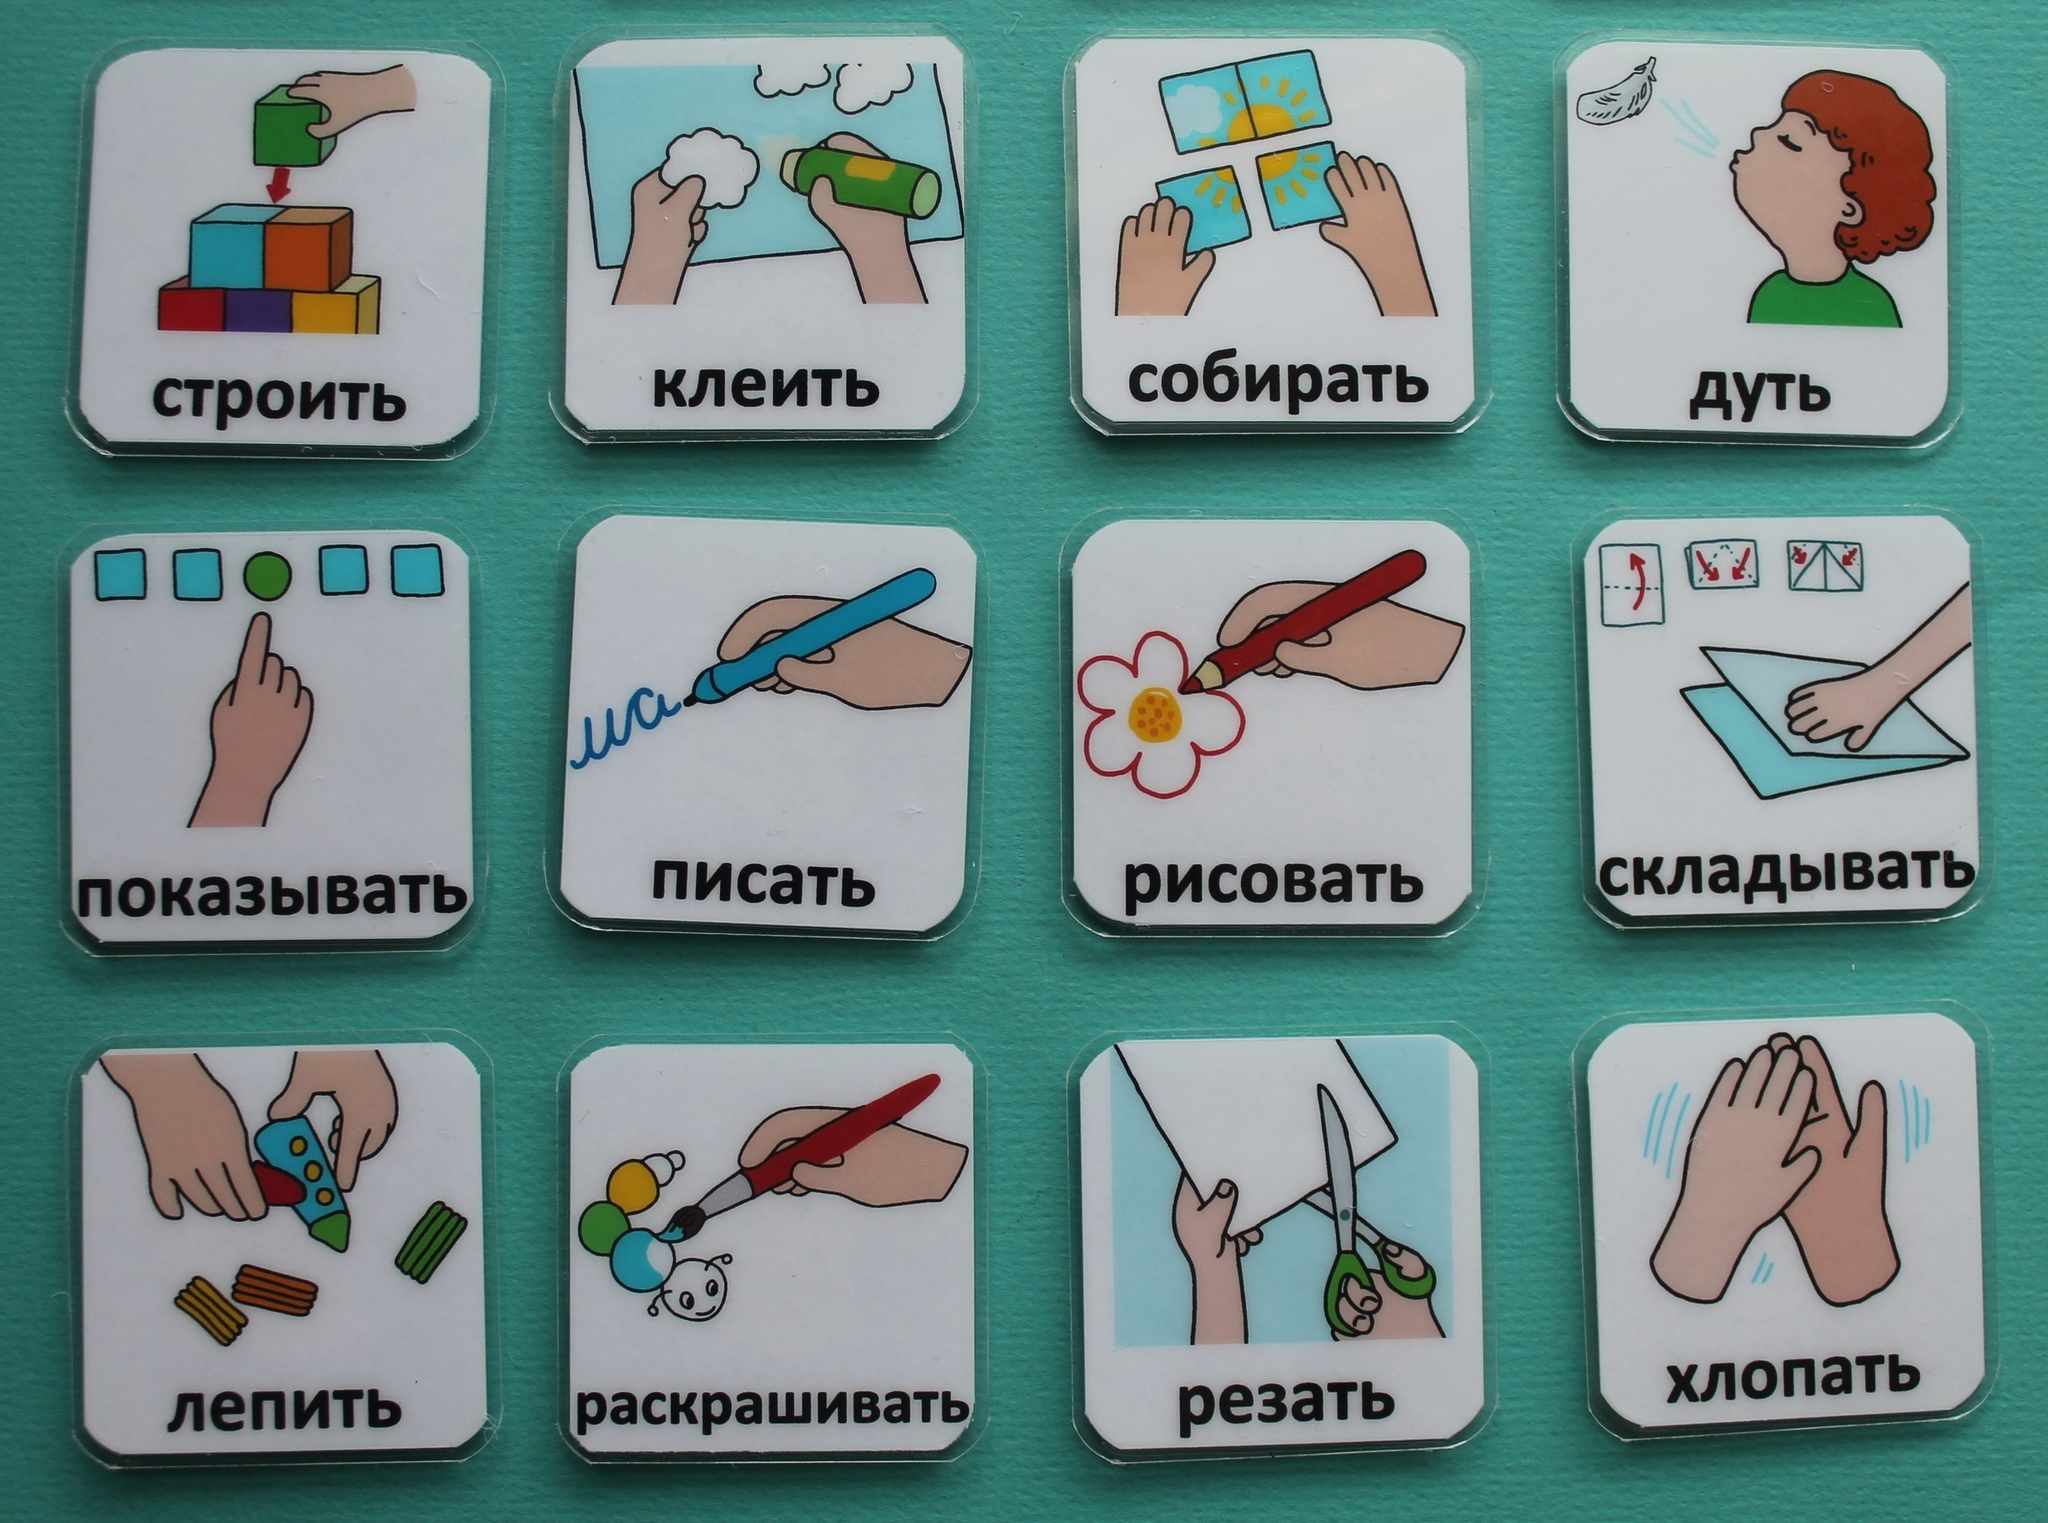
\includegraphics[scale=0.15]{PECS}
	\caption{Примеры карточек PECS}
	\label{PECScards}
\end{figure}

Программа PECS разработана в прошлом веке в конце 80-х годов доктором Э. Бонди в тесном сотрудничестве с логопедом Л. Фрост. После появления первой версии программа постоянно совершенствуется. Сегодня система PECS приспособлена для обучения не только детей с аутизмом, но также пациентов любых возрастных категорий с коммуникационными и речевыми проблемами.

\section{Пользователи системы}

В системе должно быть три уровня пользователей:
\begin{enumerate}[label=\arabic*.]
	\item Психолог --- пользователь, обладающий возможностями изменять, добавлять, удалять и просматривать сущности базы данных;
	\item Пациент --- пользователь, обладающий возможностью только просматривать сущности базы данных.
	\item Родственник --- пользователь, обладающий возможностями изменять и просматривать сущности базы данных;
\end{enumerate}

На рисунке \ref{users} представлена диаграмма вариантов использования.

\begin{figure}[ht!]\centering
	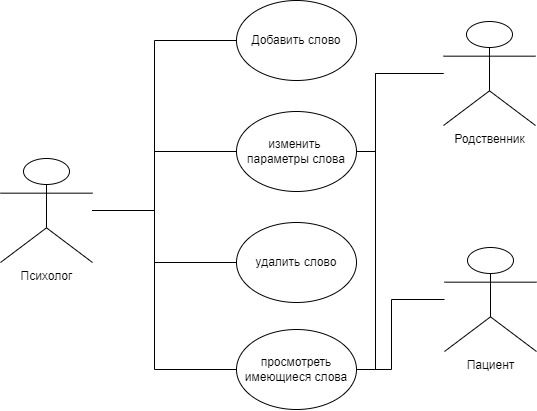
\includegraphics[scale=0.51]{usecase}
	\caption{Диаграмма вариантов использования}
	\label{users}
\end{figure}

\pagebreak

Основной пользователь приложения, то есть пользователь с ролью <<Пациент>> может использовать базу данных для разных целей:
\begin{enumerate}[label=\arabic*.]
	\item составление расписания --- пользователю необходимо чётко обозначать план действий на ближайший день, что реализуется с помощью последовательности из карточек PECS;
	\item составление истории --- пользователь использует карточки PECS для составления рассказа, несколько карточек помещаются на одну большую карту, обозначающую место действия, вместе карточки образуют непрерывную историю;
	\item взаимодействие с глобальной сетью Интернет --- пользователь с помощью карточек PECS создаёт запрос в сеть, который обрабатыватся и преобразуется в ответ поисковой системы, представленный также карточками PECS;
\end{enumerate}



\section{Описание данных}

База данных будет состоять из 5 таблиц:
\begin{enumerate}[label=\arabic*.]
	\item таблица владельцев словарей Owner;
	\item таблица главных слов <<Термин>>;
	\item таблица действий субъекта <<Действие субъекта>>;
	\item таблица действий объекта <<Действие объекта>>;
	\item таблица характеристик <<Характеристика>>.
\end{enumerate}

Каждая таблица описывает сущность базы данных, к которым будут прилагаться поля, хранящие в себе информацию о данной сущности.

На рисунке \ref{chen} представлена ER-диаграмма в нотации Чена.

\pagebreak

\begin{figure}[ht!]\centering
	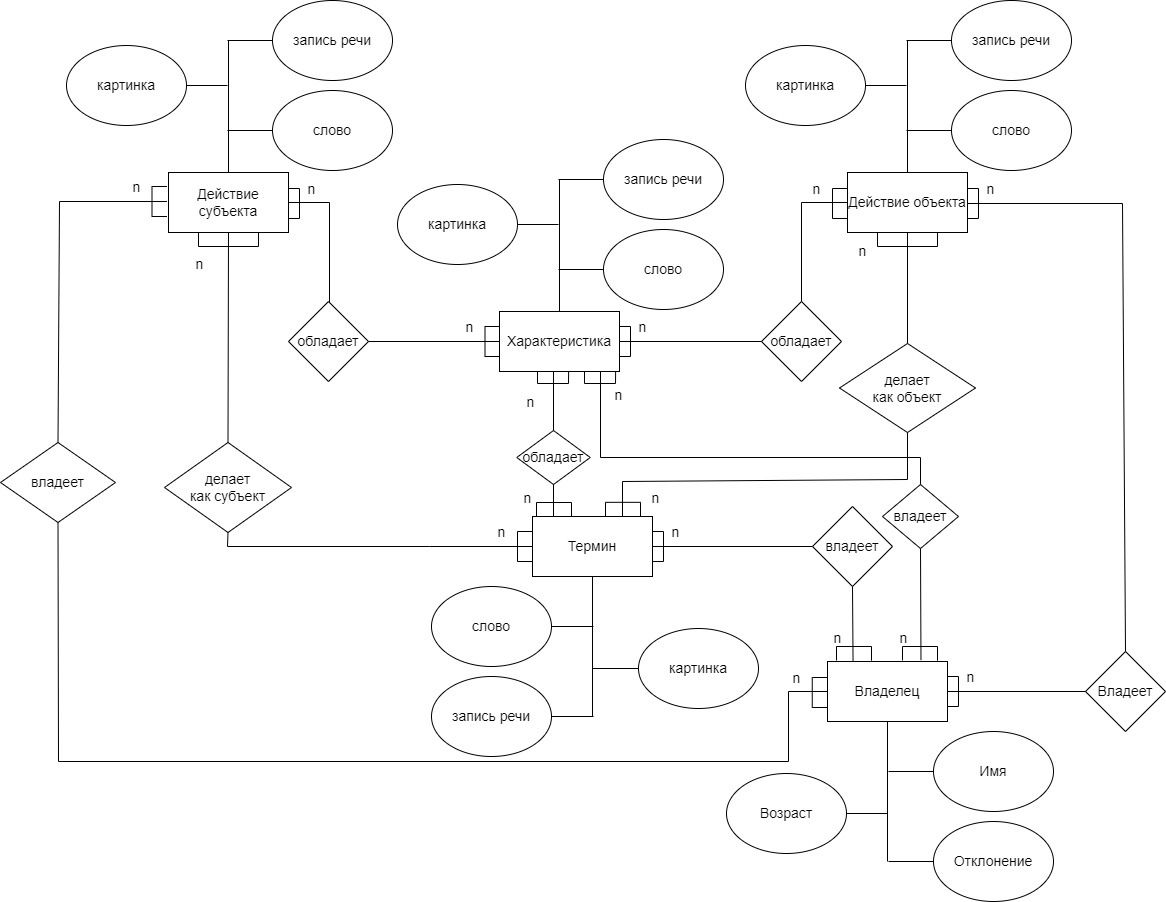
\includegraphics[scale=0.35]{Chen}
	\caption{ER-диаграмма в нотации Чена}
	\label{chen}
\end{figure}

\section{Выбор модели БД}

Основываясь на представлении данных в данной работе будет использоваться графовая нереляционная модель. Такой подход обладает следующими характеристиками:
\begin{enumerate}[label=\arabic*.]
	\item отсутствие развязочных таблиц;
	\item произвольный доступ к данным;
	\item исключение дублирования за счёт множественных связей.
\end{enumerate}

\section*{Вывод}

В данном разделе был проведён анализ предметной области, описаны карточки для адаптивного общения, а также приведена классификация существующих СУБД. Выбраны пользователи системы, описан вид хранения данных и приведены соответствующие диаграммы.